\documentclass[11pt]{article}

\usepackage{comment} % enables the use of multi-line comments (\ifx \fi) 
\usepackage[a4paper,margin=1cm]{geometry}
\usepackage[utf8]{inputenc}
\usepackage[ngerman]{isodate}
\usepackage{gensymb}
\usepackage{graphicx}
\usepackage{booktabs}% http://ctan.org/pkg/booktabs
\usepackage{tabularx}
\usepackage{ltablex} % Longtables with tabularx
\usepackage[x11names]{xcolor}
\usepackage{amsmath}
\usepackage{amssymb}
\usepackage{amsthm}
\usepackage{array}
\usepackage{wrapfig}
\usepackage{subcaption}
\usepackage{csquotes}
\usepackage{lscape}
\usepackage{geometry}
\usepackage{multicol}
\usepackage{bm}
\usepackage{enumitem}
\usepackage{hyperref}
\usepackage{mdframed}
\usepackage{scalerel}
\usepackage{stackengine}
\usepackage{mathtools}
\usepackage{pdfpages}

% Code highlighting
\usepackage{minted}
\surroundwithmdframed{minted}

% Be able to caption equations and float them in place
\usepackage{float}

\newmdtheoremenv{theorem}{Theorem}

\theoremstyle{definition}
\newmdtheoremenv{definition}{Definition}[section]


\geometry{a4paper, margin=2.4cm}

\newcommand\equalhat{\mathrel{\stackon[1.5pt]{=}{\stretchto{\scalerel*[\widthof{=}]{\wedge}{\rule{1ex}{3ex}}}{0.5ex}}}}
\newcommand\defeq{\mathrel{\overset{\makebox[0pt]{\mbox{\normalfont\tiny def}}}{=}}}
\newcolumntype{C}{>{\centering\arraybackslash}X}

\newcommand*\samplemean[1]{\overline{#1}}
\newcommand*\ev[1]{\mathrel{\text{E}\left[#1\right]}}
\newcommand*\R{\mathbb{R}}
\newcommand*\Z{\mathbb{Z}}
\newcommand*\N[1]{\mathcal{N}\left(#1\right)}
\newcommand*\F[1]{\mathcal{F}_{#1}}
\newcommand*\Likelihood{\mathcal{L}}
\newcommand*\diff{\mathop{}\!\mathrm{d}}
\newcommand*\Diff[1]{\mathop{}\!\mathrm{d^#1}}
\newcommand*\Exp[1]{\mathop{\text{Exp}}\left(#1\right)}
\newcommand*\Cov[1]{\mathop{\text{Cov}}\left(#1\right)}
\newcommand*\Cor[1]{\mathop{\text{Cor}}\left(#1\right)}
\newcommand*\Var[1]{\mathop{\text{Var}}\left(#1\right)}
\newcommand*\predvar[1]{{\color{SeaGreen4} \texttt{#1}}}

\DeclarePairedDelimiter\abs{\lvert}{\rvert}
\DeclarePairedDelimiter\norm{\lVert}{\rVert}

\setcounter{tocdepth}{3}
\setcounter{secnumdepth}{3}

\graphicspath{{./img/}}

\begin{document}
	
\title{Predictive Modelling FS20}
\author{Pascal Baumann\\pascal.baumann@stud.hslu.ch}
\maketitle



For errors or improvement raise an issue or make a pull request on the \href{https://github.com/KilnOfTheSecondFlame/mse_summaries}{github repository}.

\tableofcontents
\newpage



\section{Introduction}
Statistical Modelling means finding a density function that produces your given data. From Wikipedia:

"Predictive modeling uses statistics to predict outcomes. Most often the event one wants to predict is in the future, but predictive modelling can be applied to any type of unknown event, regardless of when it occurred. In many cases the model is chosen on the basis of detection theory to try to guess the probability of an outcome given a set amount of input data."

Predictive modelling is done with Supervised Models, the major challenge in using data to make predictions is distinguishing what is a meaningful signal from the noise.

\section{Continuous Random Variables}
The set of all possible outcomes of a random experiment is called sample space $\omega$. Random variables $X$ are real-valued functions on $\omega$. $W_X$ is the value range, that is the set of all values which $X$ can take on. If $W_X$ is discrete then $X$ is called a \emph{discrete} random variable. A probability mass function (PMF) is the probability that $X$ takes on a given value and is written as $P(X=k)$, a probability distribution is the cumulative PMF for all values $x$ in $W_X$.

\subsection{Properties of Probability Density Functions}
\begin{enumerate}
	\item $f(x) \geq 0\quad \text{for all }x$
	\item $P(a<X\leq b) = F(b) - F(a) = \int_{a}^{b}f(x) dx\quad \text{area between }a \text{ and }b \text{ under }f(x)$
	\item $ \int_{-\infty}^{\infty}f(x) dx = 1$
\end{enumerate}

\begin{definition}
	The \textbf{expected value} of a continuous random variable is defined as
	\begin{equation*}
			\ev{X} = \int_{-\infty}^{\infty} x\cdot f(x) dx
	\end{equation*}
	The \textbf{variance} of a continuous random variable is defined as
	\begin{equation*}
		\text{Var}(X) = \sigma_X^2 = \ev{((X - \ev{X})^2} = \int_{-\infty}^{\infty} (x - \ev{X})^2 f(x) dx = \ev{X^2} - \ev{X}^2
	\end{equation*}
	A \textbf{quantile} $q(\alpha) (0<\alpha<1)$ of a continuous random variable $X$, respectively of a probability distribution is defined as
	\begin{equation*}
		P(X\leq q(\alpha)) = \alpha \Leftrightarrow F(q(\alpha)) = \alpha \Leftrightarrow q(\alpha) = F^{-1}(\alpha)
	\end{equation*}
\end{definition}

\begin{center}
	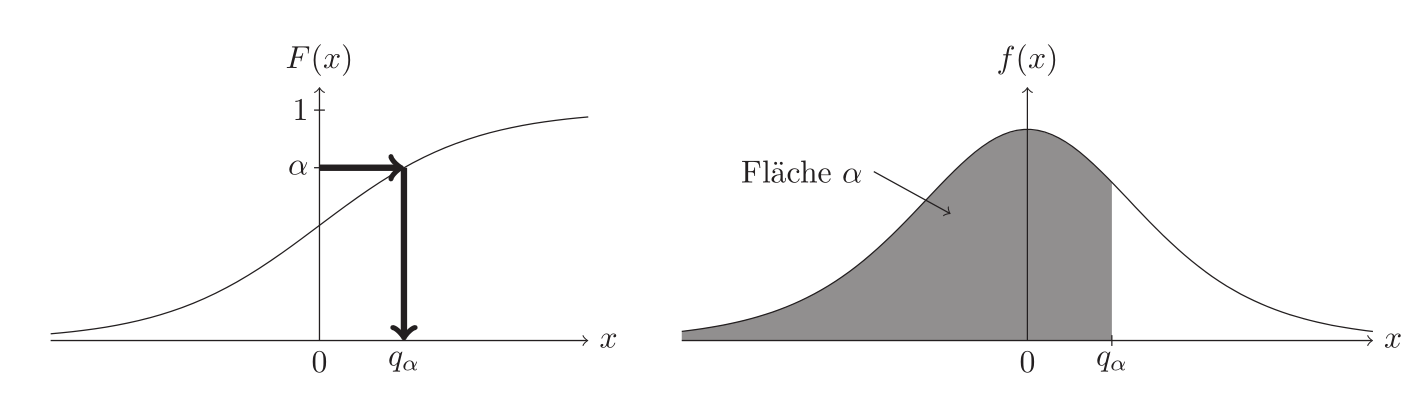
\includegraphics[width=0.8\linewidth]{img/quantile}
\end{center}

\begin{definition}
	The \textbf{sample total} is defined as 
	\begin{equation*}
		S_n = (X_1 + X_2 + \dots + X_n) \sim \N{n\mu, n\sigma_X^2}
	\end{equation*}
	\textbf{Sample mean} is defined by
	\begin{equation*}
		\samplemean{X}_n = \frac{S_n}{n} \sim(\mu, \frac{\sigma_X^2}{n})
	\end{equation*}
	\textbf{Law of Large Numbers} states that
	\begin{equation*}
		\samplemean{X}_n \longrightarrow \mu(n\rightarrow \infty)
	\end{equation*}
\end{definition}

\subsection{Uniform Distribution}
The uniform distribution represents a probabilistic formulation of complete lack of bias or knowledge
\begin{definition}
	A random variable $X$ with range $W_X = [a,b]$ is uniformly distributed if
	\begin{equation*}
		f(x) = \left\{
			\begin{matrix}
				\frac{1}{b-a} & \text{if } a\leq x \leq b\\
				0 & \text{otherwise}
			\end{matrix}
		\right.
	\end{equation*}
\end{definition}
The density function is therefore constant on the interval $[a,b]$, hence the name \emph{uniform}. The corresponding cumulative distribution function is given by
\begin{equation*}
	F(x) = \left\{
		\begin{matrix}
			0 & \text{if } x < a\\
			\frac{x-a}{b-a} & \text{if } a\leq x \leq b\\
			1 & \text{if } x > b
		\end{matrix}
		\right.
\end{equation*}

\subsection{Exponential Distribution}
The exponential distribution is used to model the lifespan or time until failure
\begin{definition}
	A random variable $X$ with range $W_X = \R^+ = [0,\infty)$ is exponentially distributed with parameter $\lambda \in \R^+$ if
	\begin{equation*}
		f(x) = \left\{
			\begin{matrix}
			\lambda\cdot e^{-\lambda x} & \text{if } x\geq 0\\
			0 & \text{otherwise}
			\end{matrix}
		\right.
	\end{equation*}
\end{definition}
The corresponding cumulative distribution function is given by
\begin{equation*}
		F(x) = \left\{
		\begin{matrix}
			1 - e^{-\lambda x} & \text{if } x\geq 0\\
			0 & \text{if } x < 0
		\end{matrix}
	\right.
\end{equation*}

\subsection{Normal Distribution}
The normal distribution or Gaussian distribution is the most frequent distribution occurring with measurement values.
\begin{definition}
	A random variable $X$ with range $W_X = \R$ is normally distributed with parameter $\mu \in \R$ and $\sigma^2\in\R^+$ if
	\begin{equation*}
	f(x) = \frac{1}{\sqrt{2\pi} \sigma} e^{\left( -\frac{(x-\mu)^2}{2\sigma^2} \right)}
	\end{equation*}
	The distribution for the random variable $X$ is denoted as follows
	\begin{equation*}
		X \sim \N{\mu,\sigma^2}
	\end{equation*}
\end{definition}

\subsubsection{Standardisation of A Normally Distributed Random Variable}
\begin{definition}
	For a random variable $ X\sim\N{\mu,\sigma^2} $, standardising $X$ results in a transformed random variable that is normally distributed as well. The expected value of this transformed variable becomes zero and the variance one. We thus obtain the standard normal distribution
	\begin{equation*}
		Z = \frac{X - \mu}{\sigma} \sim \N{0,1}
	\end{equation*}
\end{definition}

\subsection{Law Of Large Numbers}
Assume there are random variables $X_1,X_2,\dots,X_n$ i.i.d., then
\begin{align*}
	\ev{S_n} &= \ev{X_1 + X_2 + \dots + X_n} = \sum_{i=1}^{n} \ev{X_i} = n\mu\\
	\Var{S_n} &= \sum_{i=1}^{n}\Var{X_i} = n\Var{X_i} = n\sigma_X^2\\
	\sigma(S_n) &= \sqrt{n}\sigma_X
\end{align*}
The summary statistics of $\samplemean{X}_n$ thus are
\begin{align*}
	\ev{\samplemean{X}_n} &= \ev{\frac{X_1 + X_2 + \dots + X_n}{n}} = \frac{1}{n} \sum_{i=1}^{n} \ev{X_i} = \mu\\
	\Var{\samplemean{X}_n} &= \Var{\frac{X_1 + X_2 + \dots + X_n}{n}} = \frac{1}{n^2} \sum_{i=1}^{n}\Var{X_i}  = \frac{1}{n^2}n\sigma_X^2 = \frac{\sigma_X^2}{n}\\
	\sigma_{\samplemean{X}_n} &= \frac{\sigma_X}{\sqrt{n}} = \frac{1}{\sqrt{n}} \sigma_X
\end{align*}
The standard deviation of $\samplemean{X}_n$ is called \textbf{standard error} of the sample mean.
\begin{definition}
	For $n\rightarrow\infty$ the dispersion of the random variables approaches zero. If $X_1,X_2,\dots,X_n$ are i.i.d. then the \textbf{law of large numbers} applies
	\begin{equation*}
		\samplemean{X}_n \longrightarrow \mu \qquad\text{for} (n\rightarrow\infty)
	\end{equation*}
\end{definition}
The standard error is not proportional to $\frac{1}{n}$ but decreases with factor $\frac{1}{\sqrt{n}}$. Thus, to half the standard error, four times as many observations are needed, this is called the $\bm{\sqrt{n}}$-\textbf{law}.

\subsection{Central Limit Theorem}
\begin{definition}
	Let $X_1,X_2,\dots,X_n$ be i.i.d. with expected value $\mu$ and variance $\sigma^2$, then
	\begin{align*}
		S_n &\approx \N{n_\mu, n\sigma_X^2}\\
		\samplemean{X}_n &\approx \N{\mu,\frac{\sigma_X^2}{n}}
	\end{align*}
	This approximation becomes more precise the larger $n$ is. Moreover, the approximation is better, the more the distribution of the random variable $X_i$ is similar to a normal distribution $\N{\mu,\sigma_X^2}$.
\end{definition}

\section{QQ-Plots, Parameter Estimation and t-Tests}

\subsection{QQ-Plot}

A QQ-plot is the empirical quantiles calculated from the data plotted against the theoretical quantiles. If the data is normal distributed the resulting plot has a linear relationship.

\subsubsection{Normal Plot}
\begin{enumerate}[label=(\arabic*)]
	\item Data set $x_1,x_2,\dots, x_n$
	\item $\alpha_k = \frac{k-0.5}{n}\quad k=1,2,\dots,n$
	\item Theoretical Quantile $q(\alpha_k) = \Phi^{-1}(\alpha_k)$
	\item Empirical Quantile $x_{(1)}, x_{(2)},\dots, x_{(n)}$
	\item Plot $\left( q(\alpha_k), x_{(k)} \right)$
\end{enumerate}


\subsection{Parameter Estimation}
\begin{minipage}{0.6\linewidth}
	Once we have verified that a data set follows a presumed distribution, how to estimate the \textbf{parameters} of the distribution from the $n$ observations
	\begin{equation*}
		X_1 = x_1, X_2 = x_2, \dots , X_n = x_n
	\end{equation*}
	For a discrete probability distribution the probability that these $n$ observations or events actually have occurred can be expressed as
	\begin{equation*}
		P[X_1 = x_1] \cdot P[X_2 = x_2] \cdot \dots \cdot P[X_n = x_n] \equiv \prod_{i=1}^{n} P[X_i = x_i]
	\end{equation*}
	The probability that the $n$ independent random variables $x_1,x_2,\dots,x_n$ are observed, depends on the \textbf{parameter $\theta$} which needs to be \textbf{estimated}.
	The Likelihood function $\Likelihood(\theta)$ is therefore given by
	\begin{equation*}
		\Likelihood(\theta) = \prod_{i=1}^{n} P[X_i = x_i | \theta ]
	\end{equation*}
	where $P[X_i = x_i | \theta ]$ denotes the probability mass function that value $x_i$ has been observed given $\theta$.
\end{minipage}
\begin{minipage}{0.4\linewidth}
	\centering
	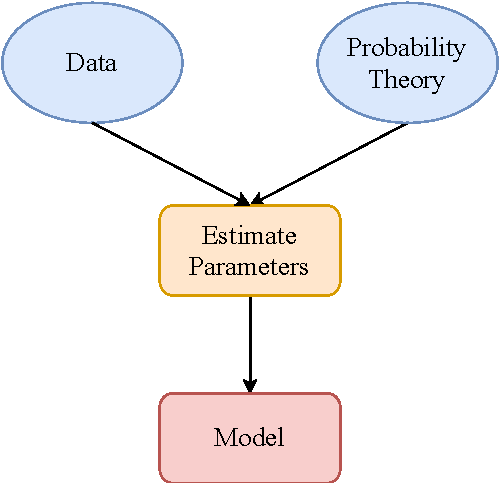
\includegraphics[keepaspectratio, width=0.8\linewidth]{probtheory_model}
\end{minipage}

The idea of \textbf{Maximum Likelihood} is to estimate the parameter $\theta$ in such a way that the \textbf{likelihood is maximised}, that is \emph{makes the observed data most likely or most probable}.

\subsection{Maximum Likelihood Continuous Distribution}
Given a continuous probability distribution  with probability density function $f (x;\theta)$, then the probability that each observation $x_i$ falls into its corresponding interval $[x_i, x_i + \text{d}x_i]$ is
\begin{equation*}
	\prod_{i=1}^{n} f(x_i; \theta) \text{d}x_i
\end{equation*}

Infinitesimal intervals $\text{d}x_i$ do not depend on parameter value $\theta$, they can thus be omitted in the \textbf{likelihood function}

\begin{equation*}
	\Likelihood = \prod_{i=1}^{n} f(x_i;\theta)
\end{equation*}

If assumed probability density function $f (x_i ;\theta)$ and parameter value of $\theta$ are correct, we expect a high probability for the actually observed data to occur, which corresponds to a \textbf{maximisation} of $\Likelihood(\theta)$.

\subsection{Maximum Likelihood for Exponential Distribution}
Given observation $X_1, X_2, \dots, X_n\text{ i.i.d. }\sim \Exp{\lambda}$, that is $f(x_i;\lambda) = \lambda e^{-\lambda x_i}$. The \textbf{likelihood function} for such a  dataset is given by
\begin{equation*}
	\Likelihood = \prod_{i=1}^{n} \lambda e^{-\lambda x_i}
\end{equation*}

The \textbf{Log likelihood} is
\begin{equation*}
	\log(\Likelihood(\lambda)) = n\log(\lambda) - \lambda\sum_{i=1}^n x_i
\end{equation*}

\subsection{z-Test}
In the z-Test the value of $\sigma_X$ is known.
\begin{enumerate}
	\item \textbf{Model} $X_i$ is a continuous measurement variable
	\begin{equation*}
		X_i, \dots, X_n \text{i.i.d.} \N(\mu, \sigma_X^2)\quad \sigma_X\text{ known}
	\end{equation*}
	\item \textbf{Null Hypothesis} $H_0: \mu = \mu_0$\\ \textbf{Alternative Hypothesis} $H_A: \mu \neq \mu_0 \text{ or } \mu < \mu_0 \text{ or } \mu > \mu_0$
	\item \textbf{Test statistic}
	\begin{equation*}
		Z = \frac{\samplemean{X}_n - \mu_0}{\sigma_{\samplemean{X}_n}} = \frac{\samplemean{X}_n - \mu_0}{\sigma_X / \sqrt{n}} = \frac{\text{observed} - \text{expected}}{\text{standard error}}
	\end{equation*}
	\textbf{Null distribution} $Z \sim \N(0,1)$
	\item \textbf{Significance Level} $\alpha$
	\item \textbf{Rejection region for test statistic}
	\begin{alignat*}{2}
		K &= (-\infty,z_{\frac{\alpha}{2}}] \cup [z_{1-\frac{\alpha}{2}}, \infty) &\quad \text{ for } H_A : \mu\neq \mu_0\\
		K &= (-\infty, z_\alpha] &\quad \text{ for } H_A : \mu < \mu_0\\
		K &= [ z_{1-\alpha}, \infty ) &\quad \text{ for } H_A : \mu > \mu_0
	\end{alignat*}
	\item \textbf{Test Statistic} Check whether the observed value of the test statistic fall into the rejection region
\end{enumerate}

\begin{definition}
	The \textbf{$p$-value} is the probability that the test statistic will take on a value that is at least as extreme (with respect to the alternative hypothesis) as the observed value of the statistic when the null hypothesis $H_0$ is true.
\end{definition}

\begin{definition}
	\textbf{$p$-value and Test Statistic}: By means of the $p$-value the test decision can be concluded directly: If the $p$-value is smaller than the significance level, then  the null hypothesis $H_0$ is rejected, otherwise it is retained. For a given significance level $\alpha$ a conclusion is drawn on the basis of the $p$-value:
	\begin{enumerate}
		\item Reject $H_0$ if $p$-value $\leq \alpha$
		\item Reject $H_0$ if $p$-value $> \alpha$
	\end{enumerate}
\end{definition}

\subsection{Example: Statistical Test for Average Body Height}
% TODO Example Average Woman's Height



\subsection{Confidence Intervals}
% TODO Confidence Interval


\section{Multivariate Probability Distributions}

\subsection{Discrete Joint Probability Distributions}
The joint distribution of two discrete random variables $X$ and $Y$, having their values in $W_X$ and in $W_Y$ respectively, is defined by the joint probability distribution of $X$ and $Y$, that is by the following probabilities
\begin{equation*}
	P(X=x, Y=y), x\in W_X, y\in W_Y
\end{equation*}
Single distributions $P(X = x)$ of $X$ and $P(Y = y)$ of $Y$ are called marginal distributions of the joint random variable $(X,Y)$. Marginal distributions can be calculated based on their joint distribution
\begin{equation*}
	P(X=x) = \sum_{y\in W_Y} P(X = x, Y = y),\qquad x\in W_X
\end{equation*}
The conditional probability of $X$ given $Y=y$ is defined as
\begin{equation*}
	P(X = x | Y = y) = \frac{P(X = x, Y = y)}{P(Y=y)}
\end{equation*}
The marginal distributions can then be expressed as follows
\begin{equation*}
	P(X=x) = \sum_{y\in W_y} P(X=x|Y=y)P(Y=y),\qquad x\in W_X
\end{equation*}
The conditional expected value of $Y$ given $X=x$ is defined as
\begin{equation*}
	\ev{Y|X=x} = \sum_{y\in W_Y} y\cdot P(Y=y|X=x)
\end{equation*}

\subsection{Joint Probability Density}
The probability that the joint random variable $(X,Y)$ lies in a two-dimensional region $A$, that is $A\subset \R^2$, is given by
\begin{equation*}
	P\left( (X,Y) \in A \right) = \iint_{A} f_{X,Y}(x,y) \diff x \diff y
\end{equation*}
This integral corresponds to the volume enclosed by by the surface of the joint density function $f_{X,Y}(x,y)$ and by the region $A$, in particular $\iint_{\R^2} f_{X,Y}(x,y) \diff x\diff y = 1$

\subsubsection{Life Expectancy of Two Machines Example}
Consider two machines with exponentially distributed life expectancy $X\sim \Exp{\lambda_1}$ and $Y\sim\Exp{\lambda_2}$, where $X$ and $Y$ are independent random variables. What is the probability that machine one runs longer than machine two?

The density functions for life expectancy of the two machines are:
\begin{equation*}
	f_X(x) = \lambda_1 e^{-\lambda_1 x}\text{ and } f_Y(y) = \lambda_2 e^{-\lambda_2 y}
\end{equation*}
Due to \textbf{independence} of the two random variables, the \textbf{joint density} can be calculated as follows
\begin{align}
	f_{X,Y} (x,y) &= f_X(x) \cdot f_Y(y)\\
	&= \lambda_1 e^{-y\lambda_1} \cdot \lambda_2 e^{-\lambda_2 y}
\end{align}
\begin{minipage}{0.6\linewidth}
	Relevant Set:
	\begin{equation*}
		A = \{(x,y)|0\leq y\leq x\}
	\end{equation*}
\end{minipage}
\begin{minipage}{0.4\linewidth}
	\begin{center}
		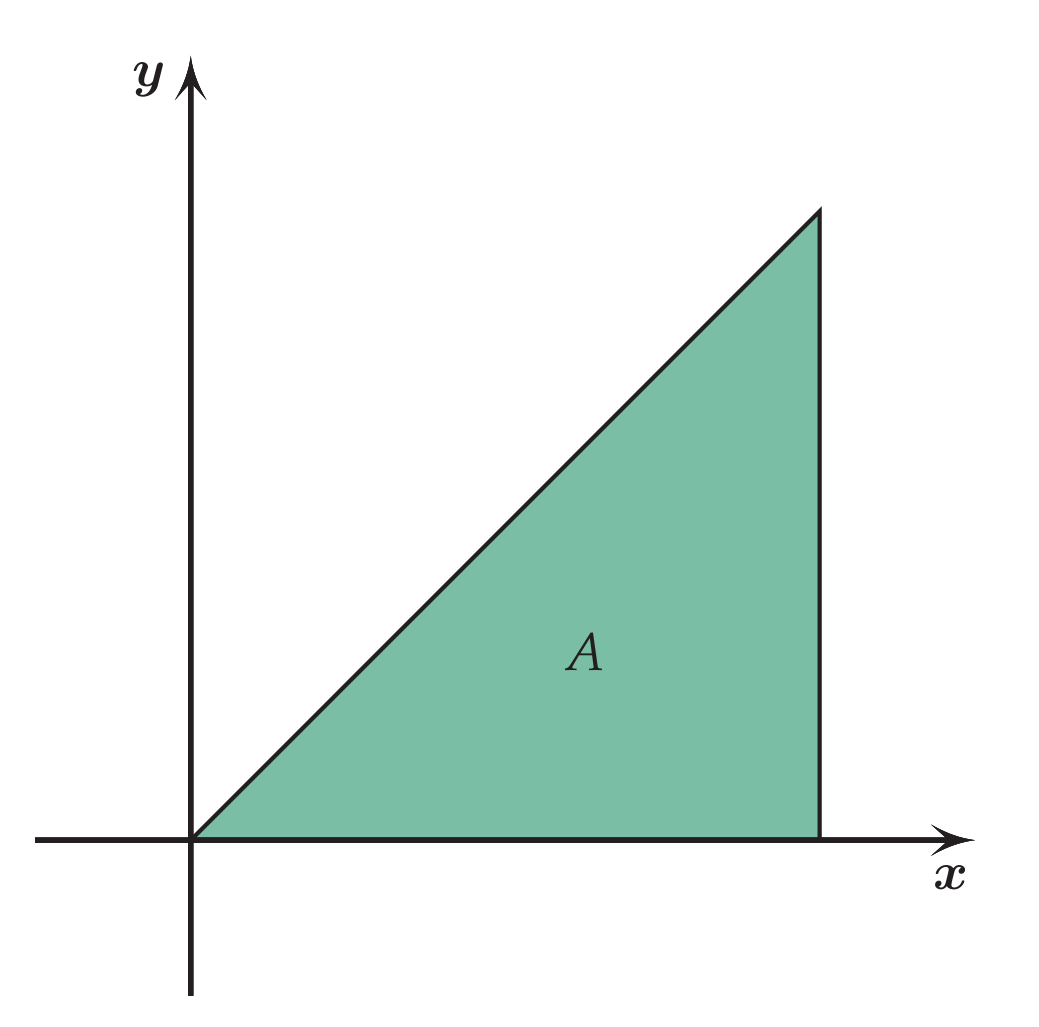
\includegraphics[width=0.6\linewidth]{img/area_A_under_xy}
	\end{center}	
\end{minipage}
Probability that machine one runs longer than machine two:
\begin{align*}
	P(Y<X) &= \int_{0}^{\infty}(\int_{0}^{x} \lambda_1 e^{-y\lambda_1} \cdot \lambda_2 e^{-\lambda_2 y} \diff y )\diff x\\
	&= \int_{0}^{\infty} \lambda_1e^{-\lambda_1 x} (1 - e^{-\lambda_2 x})\diff x\\
	&= \frac{\lambda_2}{\lambda_1 + \lambda_2}
\end{align*}

\begin{center}
	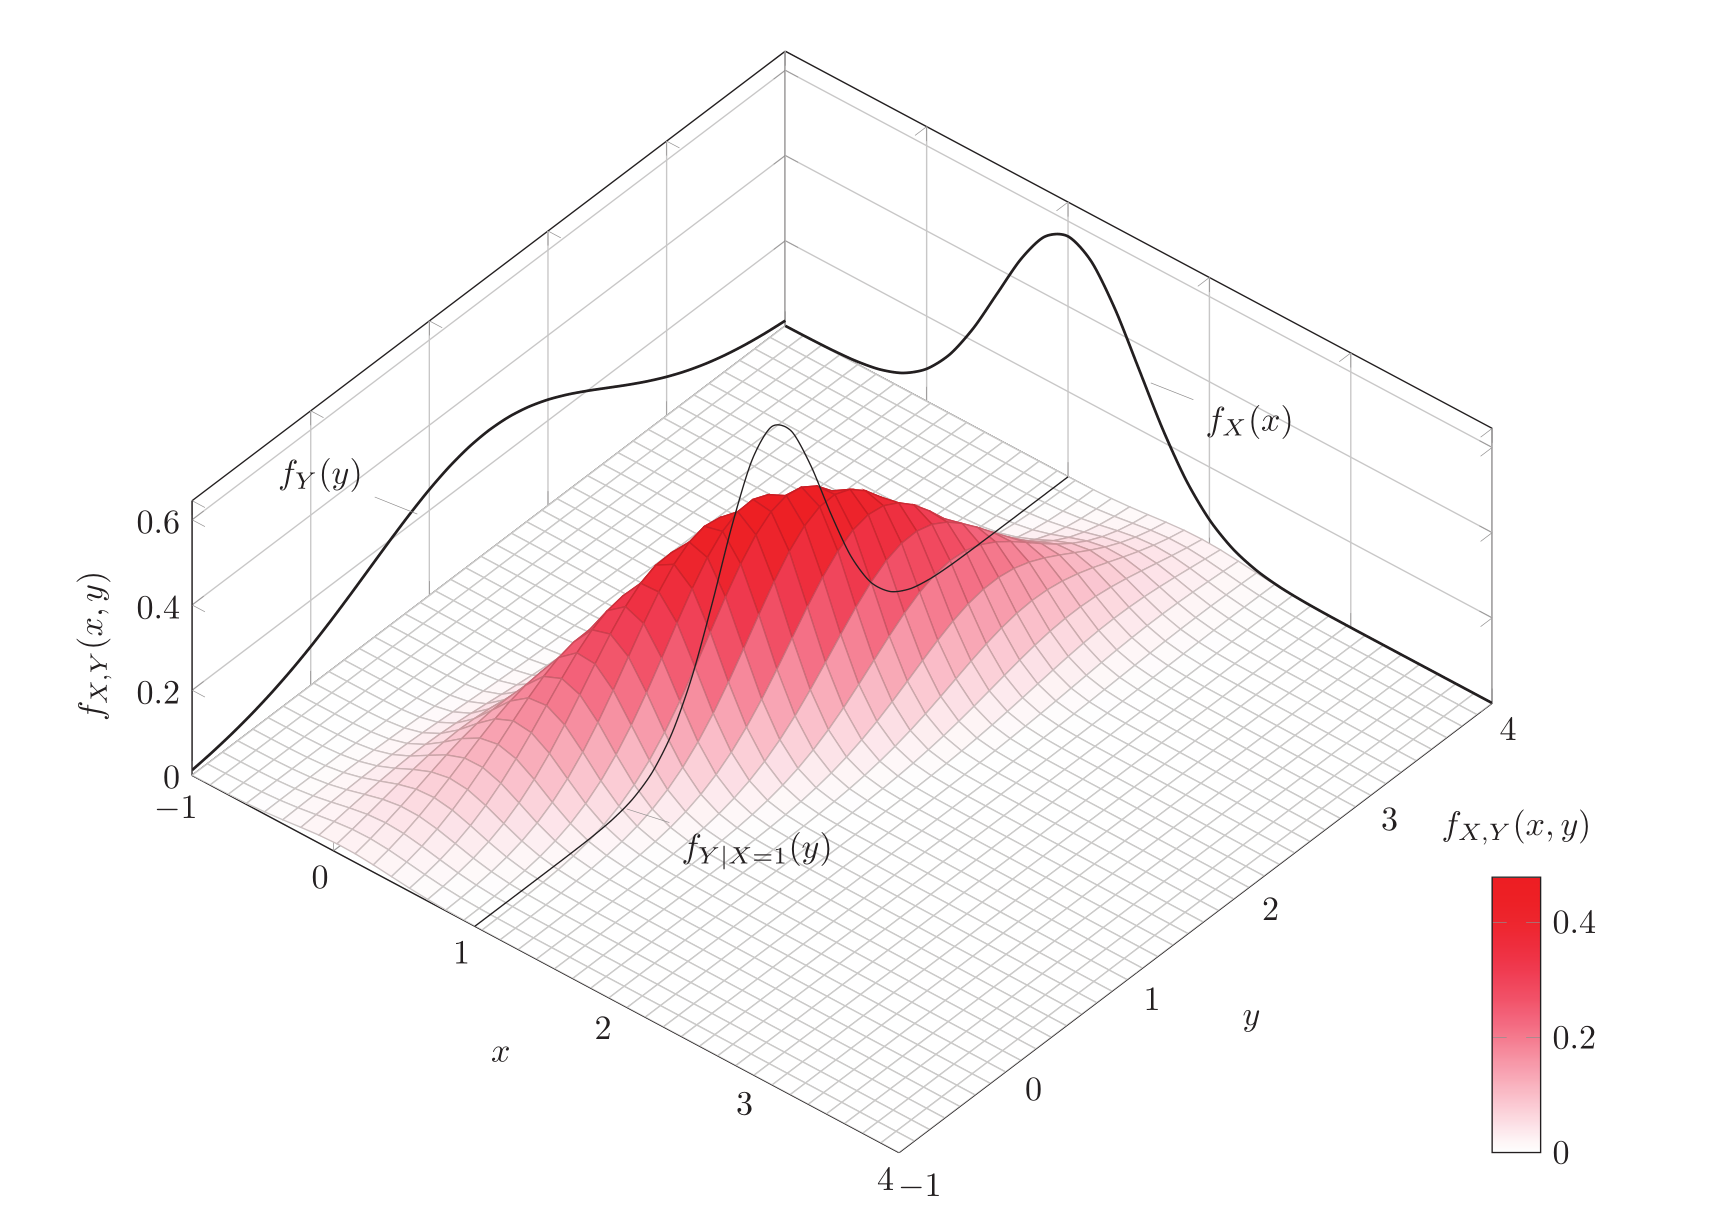
\includegraphics[width=0.8\linewidth]{img/marginal_density_xy}
\end{center}

Using the joint density, the marginal densities of $X$ and of $Y$ are obtained by integrating over the other variable
\begin{equation*}
	f_X(x) = \int_{-\infty}^{\infty}f_{X,Y}(x,y)\diff y \qquad\qquad f_Y(y) = \int_{-\infty}^{\infty}f_{X,Y}(x,y)\diff x
\end{equation*}

\begin{center}
	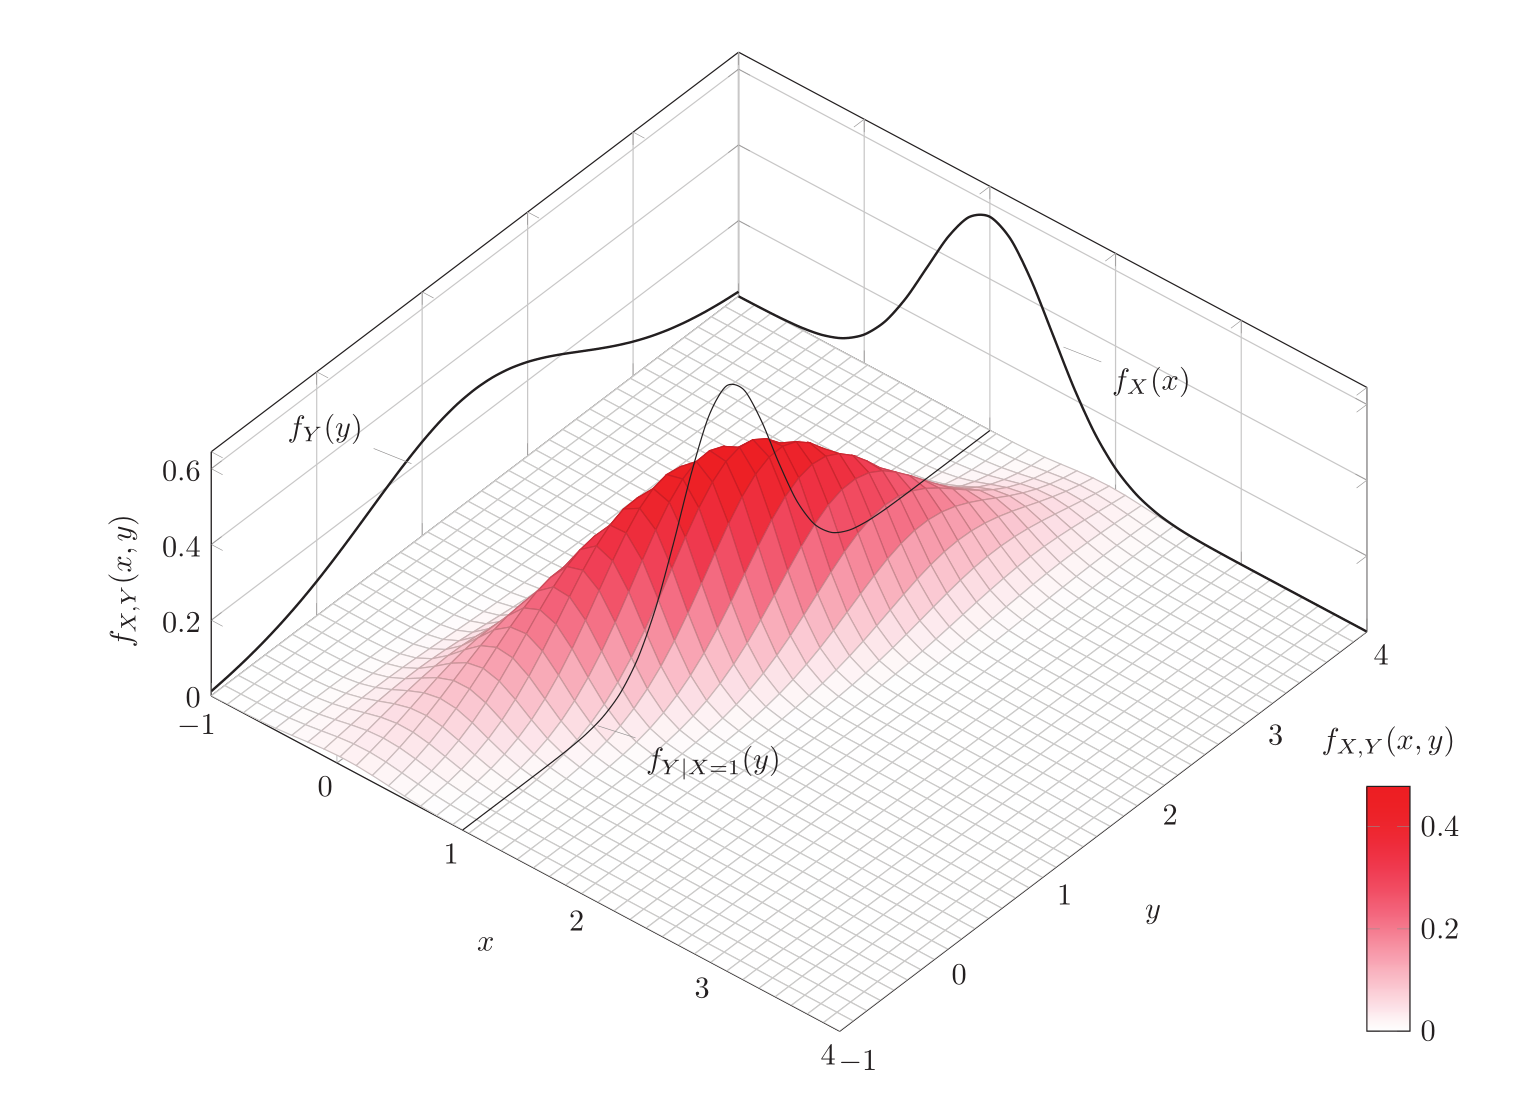
\includegraphics[width=0.8\linewidth]{img/conditional_probability_xy}
\end{center}

The conditional probability of $Y$ given $X = x$ is defined as
\begin{equation*}
	f_{(Y | X=x)} = f_Y (y | X=x) = \frac{f_{X,Y}(x,y)}{f_X(x)}
\end{equation*}
Conditional probability density corresponds to \textbf{longitudinal section} of the joint density

\subsection{Covariance and Correlation}

\subsubsection{Empirical Covariance}
\begin{minipage}{0.4\linewidth}
	\begin{center}
		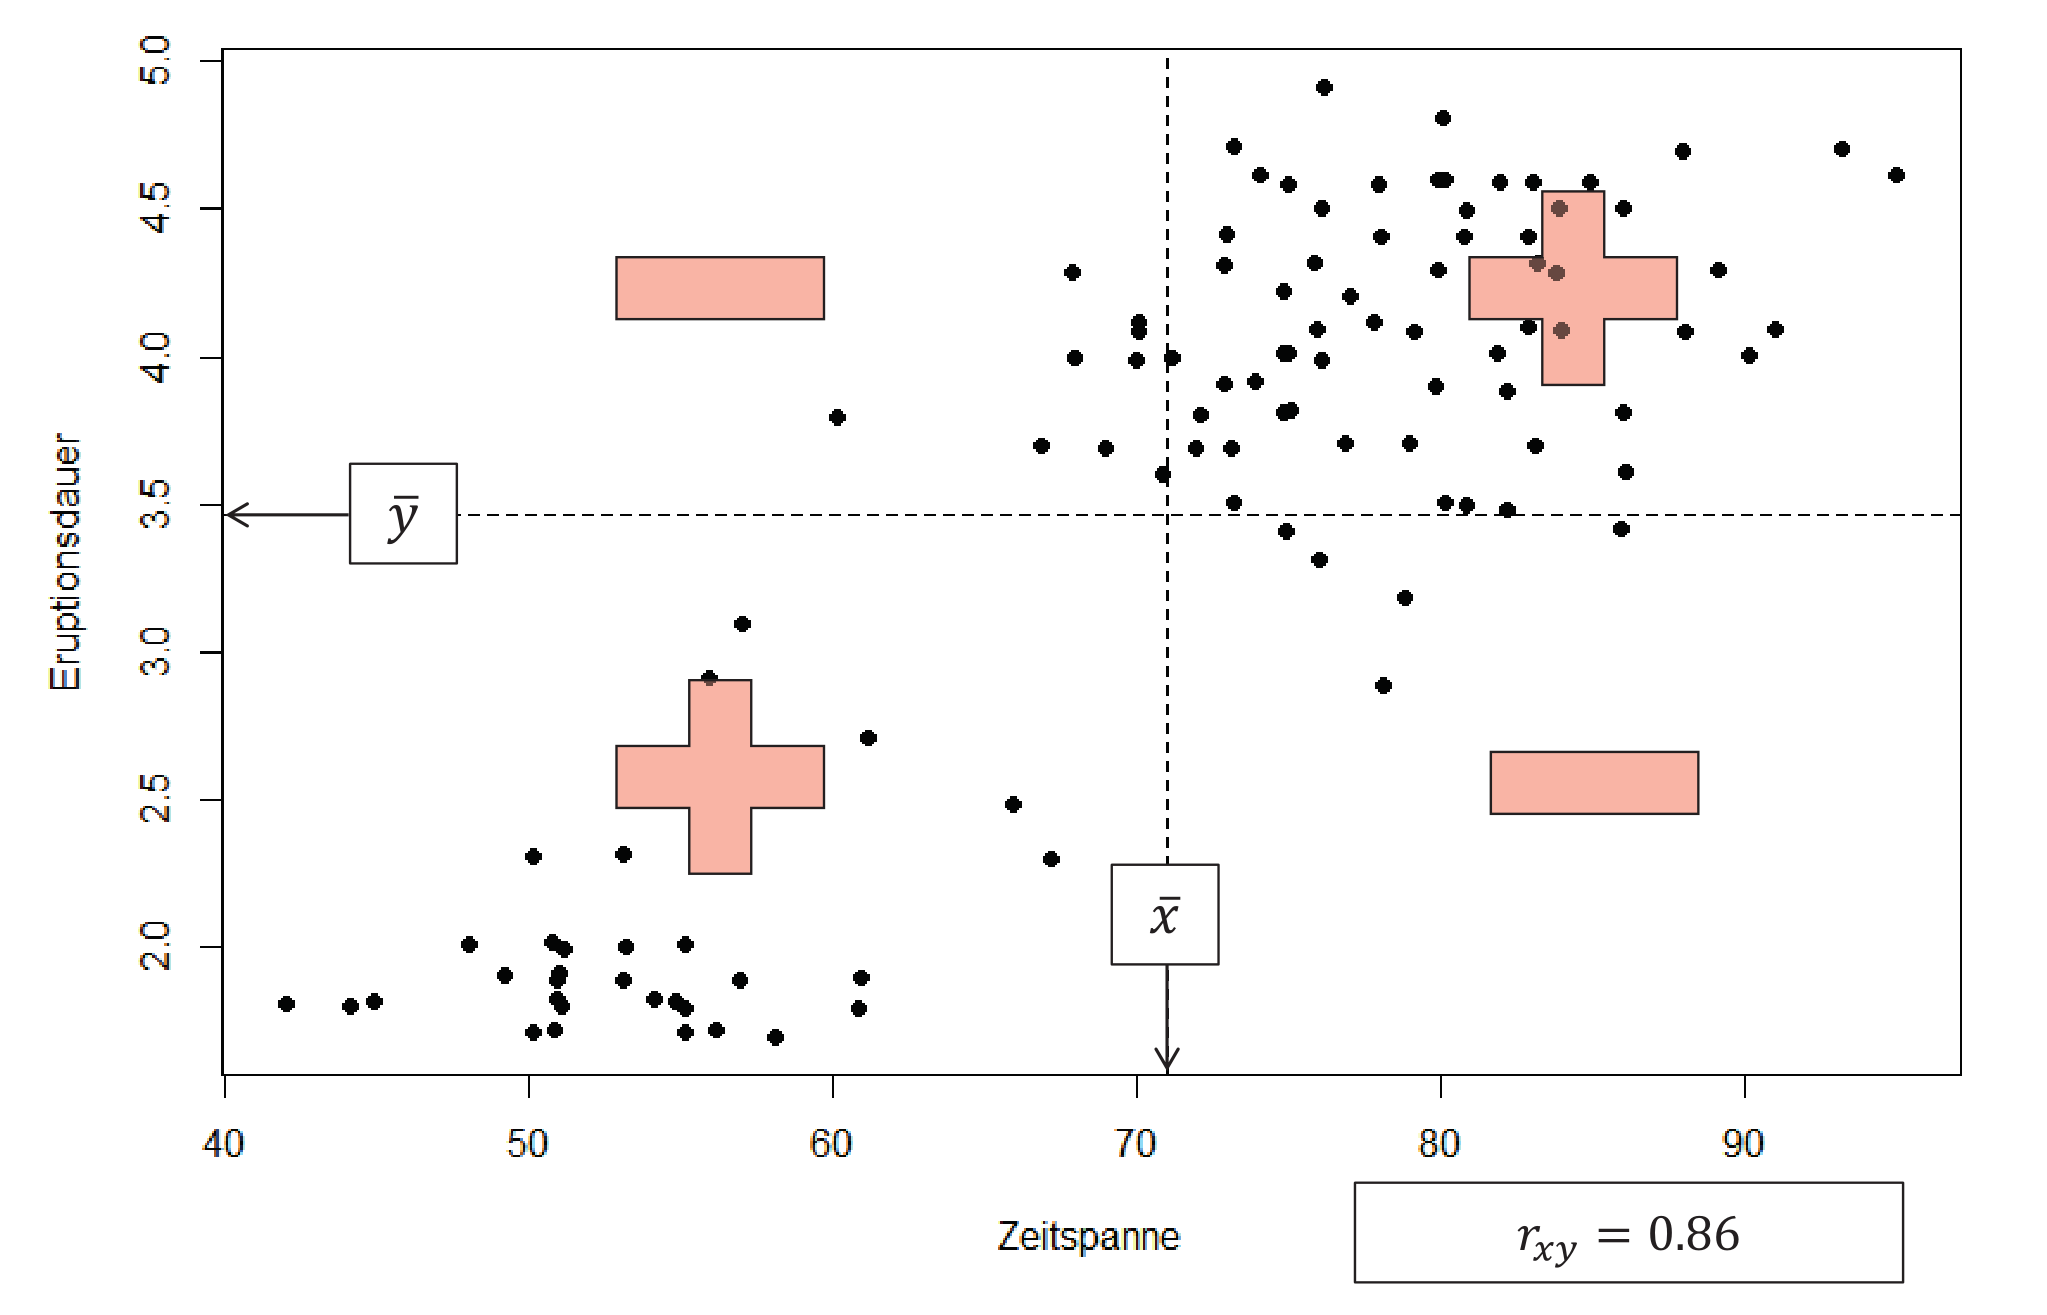
\includegraphics[width=0.9\linewidth]{img/empirical_covariance}
	\end{center}
\end{minipage}
\begin{minipage}{0.6\linewidth}
	The empirical covariance is the average value of the product of the deviation of $x_i$ from its mean $\samplemean{x}$ and the deviation of $y_i$ from its mean $\samplemean{y}$
	\begin{equation*}
		q_{xy} = \frac{1}{n-1}\sum_{i=1}^{n}(x_i - \samplemean{x} )(y-\samplemean{y})
	\end{equation*}
\end{minipage}

\subsubsection{Theoretical Covariance}
\begin{definition}
	The \textbf{covariance} of two random variables $X$ and $Y$ is defined as
	\begin{equation*}
		\Cov{X,Y} = \ev{(X-\mu_x)(Y-\mu_y)}
	\end{equation*}
\end{definition}
The covariance is the average value of the product of the deviation of $X$ from its mean $\mu_X$ and the deviation of $Y$ from its mean $\mu_Y$. If $X$ and $Y$ are \textbf{positively} associated, that is when $X$ is larger than its mean Y tends to be larger than its mean as well, the \textbf{covariance} will be \textbf{positive}. If the association between $X$ and $Y$ is \textbf{negative}, that is when $X$ is larger than its mean $Y$ tends to be smaller than its mean, the \textbf{covariance} is \textbf{negative}.

\subsection{Correlation}
\begin{definition}
	The correlation of $X$ and $Y$, denoted by $\rho$ is
	\begin{equation*}
		\Cor{X,Y} = \rho_{XY} = \frac{\Cov{X,Y}}{\sigma_X\sigma_Y}
	\end{equation*}
\end{definition}
Correlation is simply a standardized version of the covariance. Contrary to the covariance, the correlation is thus a dimensionless quantity. 

\subsubsection{Properties of the Correlation}
$\rho$ has the following property
\begin{equation*}
	-1 \leq \Cor{X,Y} \leq 1
\end{equation*}
The correlation is a measure for the strength and direction of the linear dependency between $X$ and $Y$. We have
\begin{align*}
	\Cor{X,Y} &= +1 \qquad\text{iff}\qquad Y=a+bX \text{ for $a\in\R$ and $b>0$}\\
	\Cor{X,Y} &= -1 \qquad\text{iff}\qquad Y=a+bX \text{ for $a\in\R$ and $b<0$}\\
\end{align*}
If $\abs{\Cor{X,Y}} = 1$, then there is a perfectly linear relationship between $X$ and $Y$.
\begin{figure}[tbh]
	\centering
	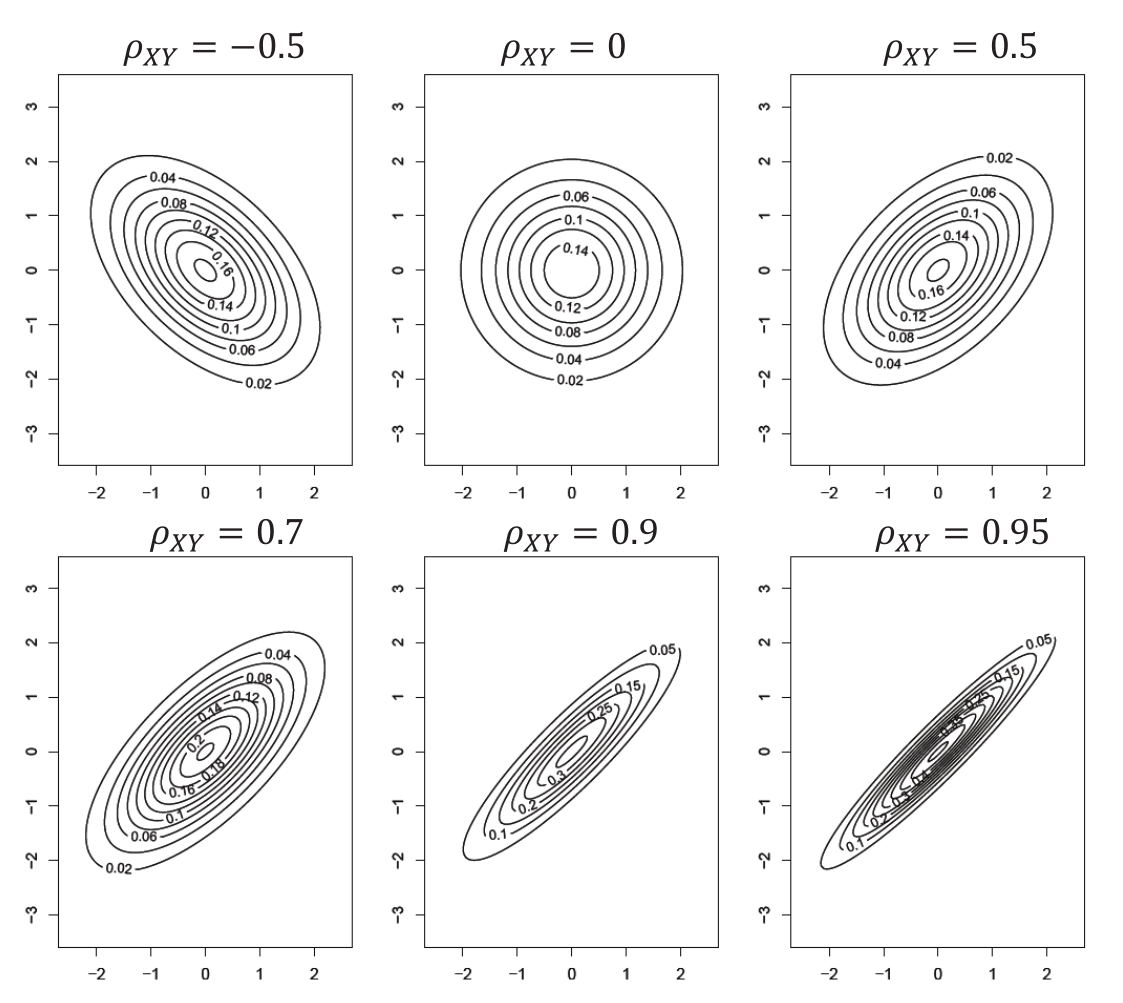
\includegraphics[width=0.6\linewidth]{img/correlation_contour_lines}
	\caption{Contour lines of bivariate normal distributions for different correlation coefficients}
	\label{fig:correlationcontourlines}
\end{figure}

\begin{definition}
	If $\Cor{X,Y}=0$ then $X$ and $Y$ are \textbf{uncorrelated}. In this case there is no linear relationship between $X$ and $Y$. There may be a non-linear relationship however.
\end{definition}

\subsubsection{Uncorrelatedness and Independence}
\begin{equation*}
	X\text{ and } Y \text{ independent} \Rightarrow \Cor{X,Y}=0\Rightarrow \Cov{X,Y}=0
\end{equation*}
However, the converse is generally not true, that is independence does not follow from uncorrelatedness.

\vspace{1em}
\noindent
These relations follow immediately from the definition of the covariance
\begin{enumerate}
	\item $\Var{X} = \Cov{X,X}$
	\item $\Cov{X,Y} = \ev{XY} - \ev{X}\ev{Y}$
	\item $\ev{XY} = \ev{X}\ev{Y}\qquad (X,Y \text{ independent})$
	\item
	\begin{equation*}
		\Var{\sum_{i=1}^{n}X_i} = \sum_{i=1}^{n}\Var{X_i} + 2\sum_{i<j}^{n}\Cov{X_i,X_j}
	\end{equation*}
	in particular in the case of two random variables
	\begin{equation*}
		\Var{X + Y} = \Cov{X + Y, X + Y} = \Var{X} + \Var{Y} + 2\Cov{X,Y}
	\end{equation*}
	\item For $X_1,\dots,X_2$ independent:
	\begin{equation*}
		\Var{X_1+\dots+X_n} = \Var{X_1} + \dots + \Var{X_n}
	\end{equation*}
\end{enumerate}

% TODO Bivariate Normal Distribution

% TODO Principal Component Analysis

\section{Simple Linear Regression}
\subsection{Regression Analysis}
Regression analysis represents a statistical method to study and model the relationship between a response variable and predictor variables. Principal goal of regression analysis is to
\begin{itemize}[noitemsep]
	\item predict data points based for some new values of the predictor variables (prediction)
	\item understand how the response variable is affected by a change of the predictor variables (inference)
\end{itemize}

\begin{center}
	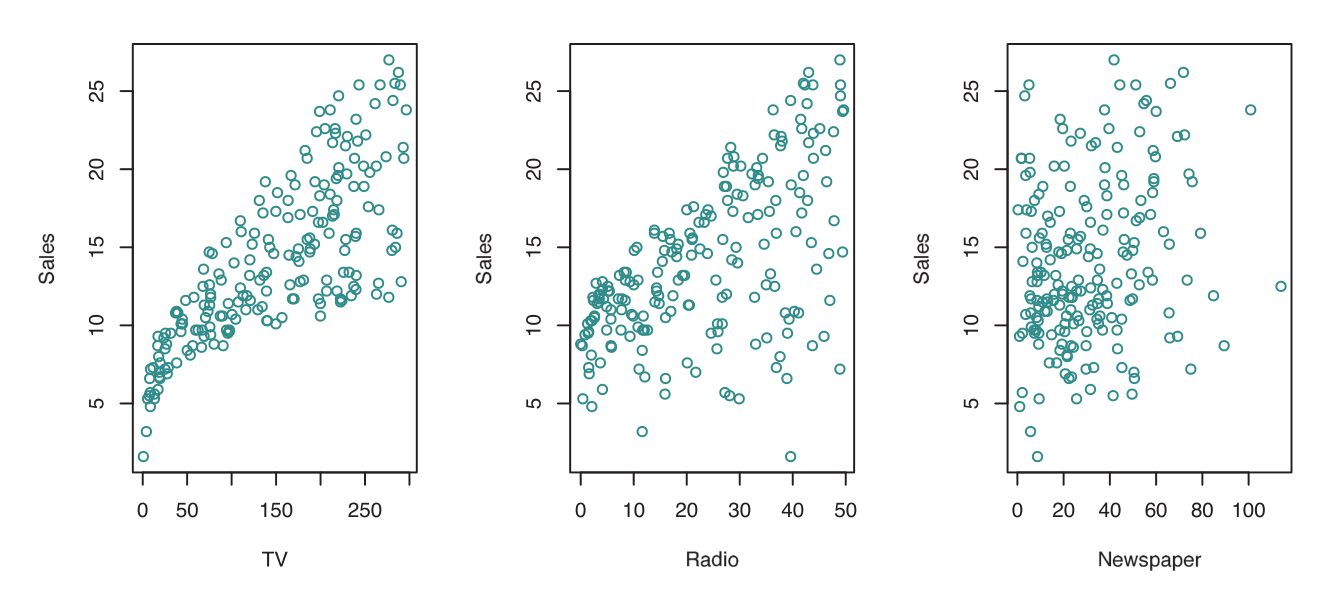
\includegraphics[width=0.8\linewidth]{img/sales_advertising}
\end{center}

The basic assumption behind this is, that there is a relationship between $Y$ and $X_1, X_2, X_3$ and deviations are random
\begin{equation*}
	Y = f(X_1, X_2,\dots, X_p) + \epsilon
\end{equation*}
\begin{itemize}
	\item $f$ is some \emph{fixed} but unknown function of $X_1, X_2,\dots, X_p$
	\item $\epsilon$ is a random error term which is independent of $X_1, X_2,\dots, X_p$ and is $\sim\N(0,r^2)$
\end{itemize}
The simple assumption is that $f$ is linear. But Linear Regression also allows to fit non-linear curves.

\subsection{Simple Linear Regression Model}
The assumption is that there is an approximately linear relationship between $X$ and $Y$
\begin{equation*}
	Y \approx \beta_0 + \beta_1 X
\end{equation*}
\begin{itemize}[noitemsep]
	\item $\beta_0$ represents the \textbf{intercept} of the regression line
	\item $\beta_1$ measures the \textbf{slope} of the regression line
	\item $\approx$ reads as "is approximately modelled as"
\end{itemize}
The coefficient estimates are denoted as $\hat{\beta}_0, \hat{\beta}_1$.

\subsection{Least Squares Method}
Let $\hat{y}_i = \hat{\beta}_0 + \hat{\beta}_1 x_i$ be the predictor for $Y$ based on the $i$th value of $X$. The $i$th residual is thus $r_i = y_i - \hat{y}_i$ and stands for the difference between the $i$th observed response value and the $i$th predicted response value of the model. The Least Squares approach chooses $\hat{\beta}_0$ and $\hat{\beta}_1$ to minimise the residual sum of squares
\begin{equation*}
	\text{RSS} = r_1^2 + r_2^2 + r_3^2 + \dots + r_n^2
\end{equation*}

\begin{definition}
	Least Squares Coefficient Estimates
	\begin{equation*}
		\hat{\beta}_1 = \frac{\sum_{i=1}^{n}(x_i - \samplemean{x})(y_i - \samplemean{y})}{\sum_{i=1}^{n}(x_i - \samplemean{x})^2}
	\end{equation*}
	\begin{equation*}
		\hat{\beta}_0 = \samplemean{y} - \hat{\beta}_1 \samplemean{x}
	\end{equation*}
	where
	\begin{equation*}
		\samplemean{x} = \frac{1}{n}\sum_{i=1}^{n} x_i\quad\text{ and }\quad\samplemean{y} = \frac{1}{n}\sum_{i=1}^{n} y_i	
	\end{equation*}
\end{definition}

\begin{definition}
	Standard Error
	\begin{equation*}
		\text{se}(\hat{\beta}_0)^2 = \sigma^2 \left( \frac{1}{n} + \frac{\samplemean{x}^2}{\sum_{i=1}^{n}(x_i - \samplemean{x})^2} \right) \quad\text{ and }\quad \text{se}(\hat{\beta}_1)^2 = \frac{\sigma^2}{\sum_{i=1}^{n}(x_i-\samplemean{x})^2}
	\end{equation*}
	where $\sigma^2 = \Var{\epsilon}$
\end{definition}
In general $\sigma^2$ (the variance of the error term) is not known, but can be estimated on the basis of the data.
\begin{equation*}
	\hat{\sigma} = \text{RSE} = \sqrt{\frac{\text{RSS}}{n-2}} = \sqrt{\frac{r_1^2 + r_2^2 + \dots + r_n^2}{n-2}}
\end{equation*}
The factor $\frac{1}{n-1}$ is chosen so that the estimate of $\sigma$ turns out \textbf{unbiased}.

\subsection{Hypothesis Test}
\begin{itemize}[noitemsep]
	\item $H_0$ There is \textbf{no} relationship between $X$ and $Y$, \quad $\beta_1 = 0$
	\item $H_A$ There is \textbf{some} relationship between $X$ and $Y$, \quad $\beta_1 \neq 0$
\end{itemize}
To test this hypothesis, it must be determined whether $\beta_1$ is sufficiently far from zero that there is confidence that $\beta_1$ is non-zero.

\subsection{The Test Statistic T}
\begin{definition}
	A 95\% confidence interval is defined as a range of values such that with a 95\% probability, the range will contain the true unknown parameter. The range is defined in terms of lower and upper limits computed from the sample of data.
\end{definition}
The 95\% confidence can be calculated by
\begin{equation*}
	\left[ \hat{\beta}_1 - t_{0.975, n-2} \cdot \text{se}(\hat{\beta}_1), \hat{\beta}_1 + t_{0.975, n-2} \cdot \text{se}(\hat{\beta}_1) \right]
\end{equation*}

\subsection{Prediction Interval}
An important task in statistics consists of predicting future observations $Y$ for a given value of $X$. Usually the variability of the fitted value $\widehat{Y}$ is not interesting, but the variability of the future observation is. This variability is called prediction interval.

There might be the temptation to use the confidence interval to indicate the interval twidehat contains a future observation for a given $x_0$. However, this interval contains the expected value of $\widehat{y}_0 = \widehat{\beta}_0 + \widehat{\beta}_1 x_0$ only with a given probability. The scatter around the regression line expressed by the error term $\epsilon$ has to be accounted for as well. Thus the prediction interval can be calculated as follows
\begin{equation*}
\text{se}(y_0)^2 = \widehat{\sigma}^2\left(1 + \frac{1}{n} + \frac{(x_0 - \samplemean{x})^2}{\sum_{i=1}^{n}(x_i - \samplemean{x})^2}\right)
\end{equation*}

\subsection{Model Assumptions for the Error Terms $\epsilon_i$}
All test and estimation methods rely on model assumptions that the error terms $\epsilon_i$ are independent and normally distributed random variables with a constant variance
\begin{equation*}
	\epsilon_i \quad \text{i.i.d.} \quad \N{0,\sigma^2}
\end{equation*}
The error term $\epsilon_i = y_i - \left( \beta_0 + \beta_1 x_i \right)$ since $\beta_0$ and $\beta_1$ are unknown. However, the residuals $r_i = y_i - \left( \hat{\beta}_0 + \hat{\beta}_1 x_i \right)$ can be determined and are relevant to estimate the standard deviation of the error terms.

\subsubsection{Residual Standard Error}
The RSE is an estimate of the standard deviation of $\epsilon$. Roughly speaking, it is the average amount that the response will deviate from the true regression line.
\begin{equation*}
	\text{RSE} = \sqrt{\frac{r_1^2 + \dots + r_n^2}{n-2}} = \sqrt{\frac{(y_1 - \hat{y}_1)^2 + \dots + (y_n - \hat{y}_n)^2}{n-2}}
\end{equation*}
\begin{equation*}
	r = \Cor{X,Y} = \frac{\sum_{i=1}^{n}(x_i - \samplemean{x})(y_i - \samplemean{y})}{\sqrt{\sum_{i=1}^{n} (x_i - \samplemean{x})}\sqrt{\sum_{i=1}^{n} (y_i - \samplemean{y})}}
\end{equation*}

\subsection{Diagnostic Tool for Testing Model Assumptions}
To identify a non-linearity of regression function $f$, that is to falsify the model assumption $\ev{\epsilon_i} = 0$, the Tukey-Anscombe-Plot can be used.\\
\paragraph{Tukey-Anscombe-Plot}
\begin{itemize}
	\item Plot the residuals $r_i = y_i - \hat{y}_i$ on the vertival axis
	\item Plot the fitted or predicted values $\hat{y}_i$ on the horizontal axis
\end{itemize}
The expectation is that the LOESS smoother is linear around 0.
\begin{center}
	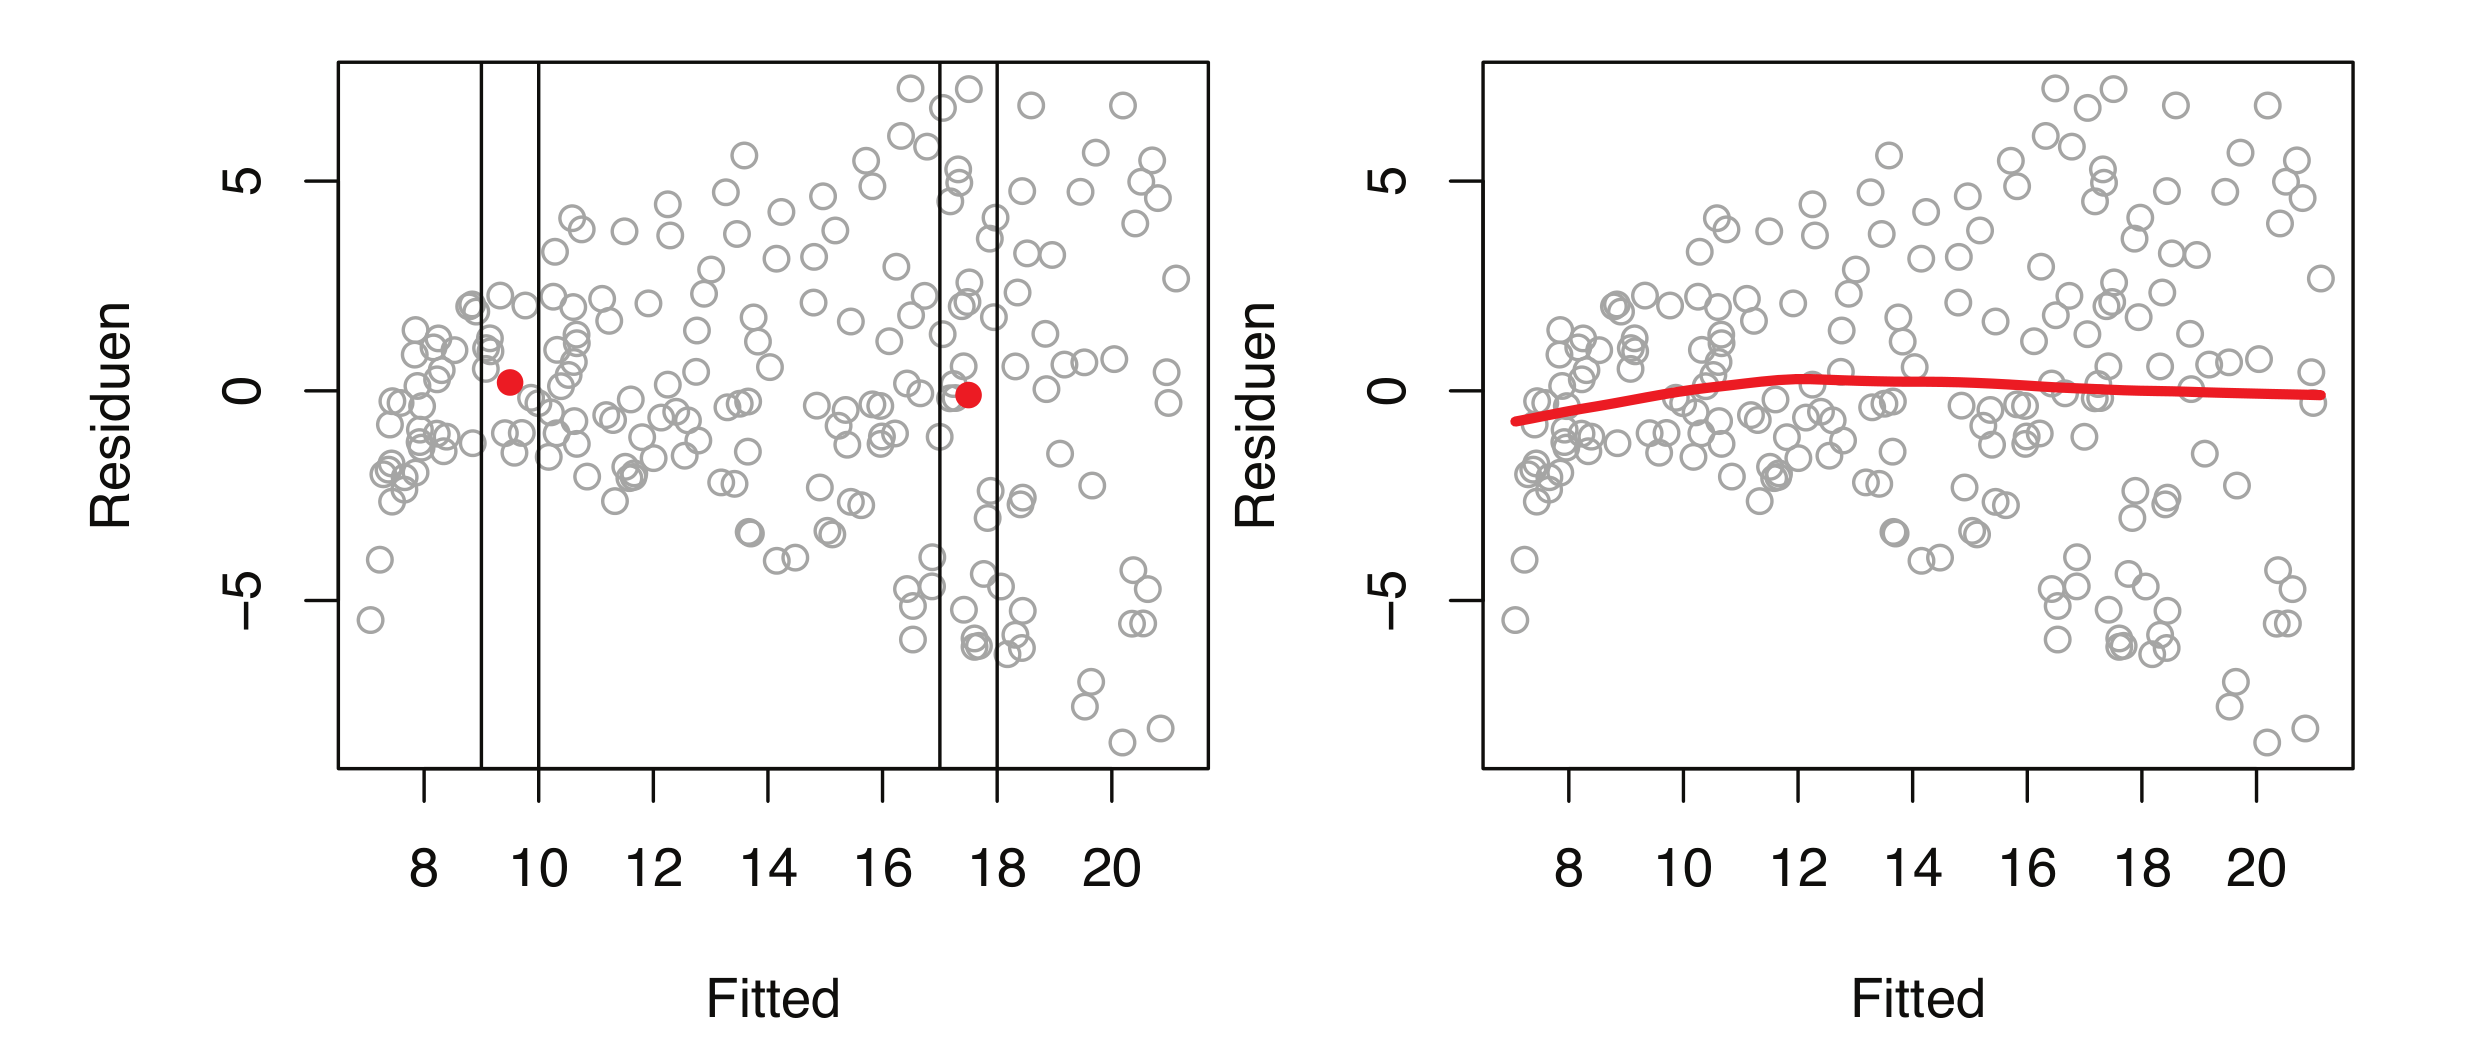
\includegraphics[width=0.8\linewidth]{img/LOESS_smoother}
\end{center}
To identify a non-constant variance in the error terms $\epsilon_i$ the standardised residuals are used
\begin{equation*}
	\tilde{r}_i = \frac{r_i}{\hat{\sigma}\sqrt{1 - \left( \frac{1}{n} + \frac{(x_i - \samplemean{x})^2}{\sum_{j=1}^{n}(x_j - \samplemean{x})^2} \right)}}
\end{equation*}
With $\hat{\sigma}$ being the estimate of the standard deviation of the error terms, and estimated by the residual standard error. If the error terms are normally distributed then $\tilde{r}_i \sim \N{0,1}$.

The resulting standardised residuals are then plotted in a so-called QQ-plot
\begin{center}
	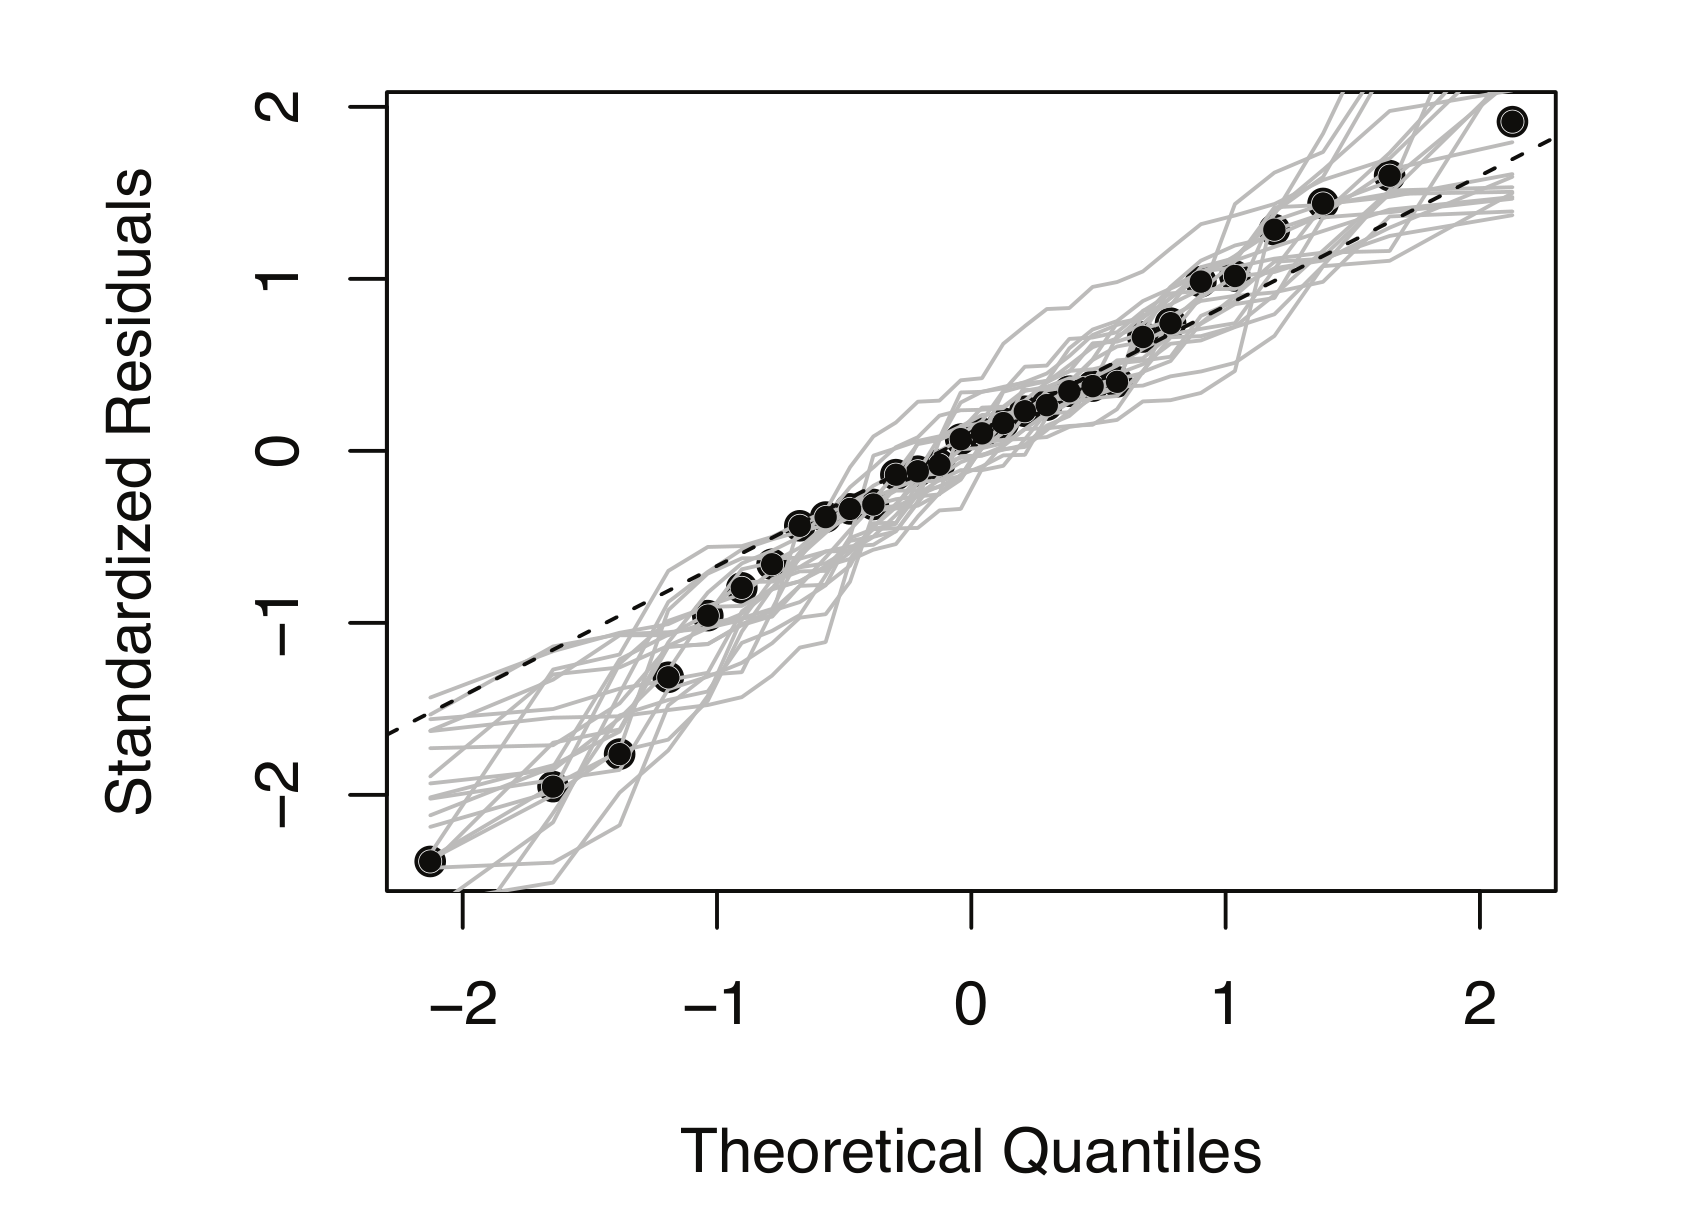
\includegraphics[width=0.5\linewidth]{img/QQ_plot}
\end{center}
\begin{theorem}
	The consequences for case of correlated error terms is that the  the estimated standard errors will tend to underestimate the true standard errors. As a result, confidence and prediction intervals will be narrower than they should be.
\end{theorem}

\subsection{Outliers}
An outlier is point for which $y_i$ is far from value $\hat{y}_i$ predicted by model. A leverage point is a point with an unusual value for $x_i$ and can be identified by the \textbf{leverage statistic}
\begin{equation*}
	h_i = \frac{1}{n} + \frac{(x_i + \samplemean{x})^2}{\sum_{i' = 1}^{n}(x_{i'}-\samplemean{x})^2}
\end{equation*}
While the Cook's distance measures the influence of an observation
\begin{equation*}
	d_i = \frac{1}{\hat{\sigma}^2}\cdot\left(\underline{\hat{y}}_{(-i)} - \underline{\hat{y}}\right)^T \left(\underline{\hat{y}}_{(-i)} - \underline{\hat{y}}\right) = \tilde{r}_i^2 \frac{h_i}{2(1-h_i)}
\end{equation*}
The larger the value of Cook’s distance $d_i$ is, the higher is the influence of the corresponding observation on the estimation of the predicted value $\hat{y}_i$. An observation with a value of Cook’s distance larger than 1 is considered as dangerously influential.

\section{Multiple Linear Regression, Qualitative Predictors and Interaction Effects}
\subsection{Multiple Linear Regression}
\begin{definition}
	\begin{equation*}
		Y = \beta_0 + \beta_1 X_1 + \beta_2 X_2 + \dots + \beta_p X_p + \epsilon
	\end{equation*}
	\begin{itemize}[label=]
		\item $X_j$ \quad $j$th predictor variable
		\item $\beta_j$ \quad association between $X_j$ and response variable $Y$
	\end{itemize}
\end{definition}

\subsection{Hypothesis Testing Using the F-Statistic}
Compute the F-Statistic as follows
\begin{equation*}
	F = \frac{\frac{\text{TSS} - \text{RSS}}{p}}{\frac{\text{RSS}}{n-p-1}} \qquad \text{TSS} = \sum_{i=1}^{n} (y_i - \samplemean{y})^2 \qquad \text{RSS} = \sum_{i=1}^{n} (y_i - \hat{y})^2
\end{equation*}
If the linear model assumptions are \textbf{correct}, it can be shown that
\begin{equation*}
	\ev{\frac{\text{RSS}}{n-p-1}} = \sigma^2
\end{equation*}
Provided the Null-Hypothesis is \textbf{true}, it can be shown that
\begin{equation*}
	\ev{\frac{\text{TSS}-\text{RSS}}{p}} = \sigma^2
\end{equation*}
That means that if there is \textbf{no} relationship between the response and the predictors, then the value of the F-Statistic is approximately 1.

When $H_0$ is true and the errors $\epsilon_i$ follow a normal distribution, the F-Statistic follows an F-distribution with $p$ and $n-p-1$ degrees of freedom.

If $H_A$ is \textbf{true}, then 
\begin{equation*}
	\ev{\frac{\text{TSS}-\text{RSS}}{p}} > \sigma^2
\end{equation*}
and the value of the F-Statistic is expected to be greater than 1.

\subsubsection{F-Test}
\begin{itemize}[label=]
	\item Null Hypothesis
	\begin{equation*}
		H_0:\quad \beta_1 = \beta_2 = \dots = \beta_p = 0
	\end{equation*}
	\item Alternative Hypothesis
	\begin{equation*}
		H_A:\quad \text{at least one $\beta_i$ is non-zero}
	\end{equation*}
	\item Assuming $H_0$ is true
	\begin{equation*}
	F = \frac{\frac{\text{TSS} - \text{RSS}}{p}}{\frac{\text{RSS}}{n-p-1}} \sim \F{p,n-p-1}
	\end{equation*}
\end{itemize}

\subsection{Factor Variable}
If a predictor variable has multiple levels, the variable gets split in multiple dummy variables. For example given a variable \predvar{ethnicity} with three levels, two dummy variables get introduced
\begin{align*}
	x_{i1} &= \left\{ \begin{matrix}1 & \text{if $i$th person is Asian}\\ 0 & \text{if $i$th person is not Asian}\end{matrix} \right.\\
	x_{i2} &= \left\{ \begin{matrix}1 & \text{if $i$th person is Caucasian}\\ 0 & \text{if $i$th person is not Caucasian}\end{matrix} \right.
	\intertext{\textbf{Regression Model}}
	y_{i} = \beta_0 + \beta_1 x_{i1} + \beta_2 x_{i2} + \epsilon_i &= \left\{ \begin{matrix}
	\beta_0 + \beta_1 + \epsilon_i & \text{if $i$th person is Asian}\\
	\beta_0 + \beta_2 + \epsilon_i & \text{if $i$th person is Caucasian}\\
	\beta_0 + \epsilon_i & \text{if $i$th person is Afro-American}
	\end{matrix} \right.\\
\end{align*}
The level without a dummy variable is known as the baseline. There are many different ways of coding qualitative variables, no effect on regression fit, but does alter interpretation of coefficients and p-values

\subsection{Interaction Effects}
Having an Additivity in the model means that the effect of changes in a predictor $X_j$ on the response $Y$ is independent of the values of the other predictors. If the changes on one predictor have an effect on another predictor, then there is an \textbf{interaction effect}.
\begin{equation*}
	\predvar{sales} = \beta_0 + \beta_1 \cdot \predvar{TV} + \beta_2\cdot\predvar{radio} + \beta_3\cdot(\predvar{TV}\cdot\predvar{radio}) + \epsilon
\end{equation*}
\begin{minted}{R}
Advertising <- read.csv('Advertising.csv', header=True)
summary(lm(sales ~ TV + radio + TV * radio, data = Advertising))
# equivalent
summary(lm(sales ~ TV * radio, data = Advertising))
\end{minted}

\section{Polynomial Regression, Residual Analysis and Model Selection}

\subsection{Polynomial Regression Model}

\begin{equation*}
	Y = \beta_0 + \beta_1\cdot X + \beta_2\cdot X^2 + \epsilon
\end{equation*}

\begin{minted}{R}
lm(Y ~ X + I(X^2), data = Data)
\end{minted}

\subsection{Identification of Collinearity}
Collinearity refers to the situation in which two or more predictor variables are closely related to one another. Collinearity can be detected by using the \textbf{correlation matrix} \mintinline{R}{cor(Data)} and the \textbf{variance inflation factor}
\begin{equation*}
	\text{VIF}(\hat{\beta}_j) = \frac{1}{1- R_{(X_j|X_{-j})}^2}
\end{equation*}
\begin{itemize}
	\item VIF $5\leq x\leq 10$: indicates a problematic amount of collinearity
	\item VIF is 1: indicates complete absence of collinearity
\end{itemize}

\subsection{Model Selection}
\subsubsection{Forward Stepwise Selection}
\begin{enumerate}
	\item Let $\mathcal{M}_0$ denote the \texttt{null} model which contains no predictors.
	\item For $k = 0,\dots,p-1$
	\begin{enumerate}
		\item Consider all $p - k$ models that augment the predictors in $\mathcal{M}_k$ with one additional predictor.
		\item Choose the \emph{best}, that is having the smallest RSS or highest $\text{R}^2$, among these $p-k$ models and call it $\mathcal{M}_{k+1}$.
	\end{enumerate}
	\item Select a single best model among $\mathcal{M}_0,\dots, \mathcal{M}_p$ using Mallow's $C_p$, Akaike's Information Criterion, Bayesian Information Criterion, or the adjusted $\text{R}^2$.
\end{enumerate}

\subsubsection{Backward Stepwise Selection}
\begin{enumerate}
	\item Let $\mathcal{M}_p$ denote the \textbf{full} model which contains all $p$ predictors.
	\item For $k = p, p-1, \dots, 1$
	\begin{enumerate}
		\item Consider all $k$ models that contains all but one of the predictors in $\mathcal{M}_k$ for a total of $k-1$ predictors.
		\item Choose the \emph{best}, that is having the smallest RSS or highest $\text{R}^2$, among these $k$ models and call it $\mathcal{M}_{k11}$.
	\end{enumerate}
	\item Select a single best model among $\mathcal{M}_0,\dots, \mathcal{M}_p$ using Mallow's $C_p$, Akaike's Information Criterion, Bayesian Information Criterion, or the adjusted $\text{R}^2$.
\end{enumerate}

\subsubsection{Selection Criterion Adjusted $\text{R}^2$}
The problem is that RSS always decreases, while $\text{R}^2$ always increases as more predictors are added to the model. The solution is to add a penalty to RSS which penalises adding more predictor variables.
\begin{equation*}
	\text{adjusted R}^2 = 1 - \frac{\frac{\text{RSS}}{(n-p-1)}}{\frac{\text{TSS}}{(n-1)}}
\end{equation*}
With $p$ being the number of predictor variables of the least squares model, and $n$ the number of data points.

To maximise the adjusted $\text{R}^2$, minimise
\begin{equation*}
	\frac{\text{RSS}}{n-p-1}
\end{equation*}

\subsubsection{Akaike's Information Criterion}
AIC considers goodness-of-fit to the data and penalises the complexity of the model
\begin{equation*}
	\text{AIC} = -2\log(L) + 2q
\end{equation*}
where $L$ denotes the value of the likelihood function for a particular model and $q$ is the number of variables of this model.

If the errors $\epsilon$ in a linear regression model follow a normal distribution with expected value $0$ and constant variance, then the AIC is
\begin{equation*}
	\text{AIC} = \frac{1}{n\cdot \hat{\sigma}^2} \left(\text{RSS} + 2p\hat{\sigma}^2\right)
\end{equation*}
\begin{itemize}[leftmargin=*, labelindent=1cm, labelsep=1cm]
	\item[$\hat{\sigma}$] estimated standard deviation
	\item[$2p\hat{\sigma}^2$] penalty term, increases if more predictors are added to the model
\end{itemize}
For the least squares model the AIC is proportional to Mallow's $C_p$-statistic
\begin{equation*}
	C_p = \frac{1}{n} (\text{RSS} + 2p\hat{\sigma}^2)
\end{equation*}

\subsubsection{Bayesian Information Criterion}
\begin{equation*}
	\text{BIC} = -2\log(L) + 2\log(n)q
\end{equation*}
where $L$ denotes the likelihood function for a particular model and $q$ is the number of estimated parameters of the model.

For the least squares model with $p$ predictors, the BIC is, apart from irrelevant constants, given by
\begin{equation*}
	\text{BIC} = \frac{1}{n}\left( \text{RSS} + log(n)p\hat{\sigma}^2 \right)
\end{equation*}


\end{document}
